\documentclass[10pt]{article}
\usepackage[a4paper,margin=1.8cm]{geometry}
\usepackage[T1]{fontenc}
\usepackage{lmodern}
\usepackage{microtype}
\usepackage{amsmath}
\usepackage{booktabs}
\usepackage{array}
\usepackage{longtable}
\usepackage{graphicx}
\graphicspath{{../supplementary/figures/}}
\makeatletter
\def\input@path{{../supplementary/}}
\makeatother
\usepackage[super,sort&compress]{natbib}
\usepackage[colorlinks=true,allcolors=blue]{hyperref}
\usepackage{enumitem}
\setlength{\parindent}{1.2em}
\setlength{\parskip}{0pt}

\title{Appendix\\[0.4em]
\large Distilling solvent response into reusable priors for simulation-free hydration prediction}
\author{Anonymous authors}
\date{}

\begin{document}
\maketitle
\tableofcontents

\section*{Supplementary Methods}
\addcontentsline{toc}{section}{Supplementary Methods}

\subsection*{S1. Reference-set processing}

The ARROW reference table was reconstructed from machine-readable project outputs and
contains 85 unique neutral solutes in water at 298 K. One molecule--condition row was
retained for each connectivity. The reference includes experimental hydration free
energy and, where available in the source, uncertainty, classical ARROW, PIMD4 and
PIMD8 values. Molecular names were not used for identity. Canonical isomeric SMILES,
full InChIKey and the first InChIKey block were generated with RDKit 2026.03.5. The
released benchmark table is \texttt{data/benchmark/arrow\_solvation\_master.parquet}.

The reconstructed ARROW/PIMD8 MAE is 0.204836 kcal mol$^{-1}$ and the classical
ARROW MAE is 0.784648 kcal mol$^{-1}$. These values are direct errors against the same
experimental column used for SolvAI evaluation; neither simulation value is an input
to the final model.

\subsection*{S2. External endpoint labels}

The endpoint-label catalog initially contained 5,075 benchmark-disjoint
connectivities. A frozen source-quality rule retained all 1,147 rows from an earlier
FreeSolv/CombiSolv-Exp merge and 133 additional SoluteML dGsolvDB3 rows supported by
at least two source measurements, giving 1,280 external labels. Duplicate structures
were resolved at the connectivity level before this rule was applied. The source
composition is listed in Supplementary Table~3. The raw merged tables are not
redistributed where source terms are not explicit; URLs, versions, hashes and
reconstruction commands are given in \texttt{repro/DATA\_PROVENANCE.md}.

For a random outer fold, these 1,280 rows were combined with the available ARROW
outer-training molecules. External rows received sample weight 1 and ARROW
outer-training rows weight 3. The experimental value of an outer-test molecule was
never used. In the zero-ARROW transfer experiment, only the 1,280 external labels
were fitted and all 85 ARROW molecules were evaluated.

The weight of 3 was part of the prospective confirmatory protocol rather than a
post-result choice. A separately committed one-factor sensitivity changed only the
available ARROW outer-training weight to 1. Under this setting, matched structure-only
and full SolvAI MAEs are 0.30977 and 0.20642 kcal mol$^{-1}$, respectively; the paired
change is -0.10335 kcal mol$^{-1}$ (95\% interval, -0.21883 to -0.01995).

\subsection*{S3. Response-source processing}

\paragraph{CombiSolv-QM.}
The water subset was deduplicated by solute connectivity and expressed in kcal
mol$^{-1}$. After the original exact-connectivity exclusion, 3,961 structures were
available. Conservative canonical-tautomer comparison found two additional
benchmark equivalents; the confirmatory teacher therefore used 3,959 rows.

\paragraph{SoluteML Abraham parameters.}
Five Abraham solute axes (E, S, A, B and L) were predicted from 8,098
benchmark-disjoint structures. These coordinates respectively describe excess molar
refraction, dipolarity/polarizability, hydrogen-bond acidity, hydrogen-bond basicity
and hexadecane--air partition response. No standardized benchmark equivalent was
found in the audited source.

\paragraph{OpenFF explicit-water response.}
The source contains 520 benchmark-disjoint absolute solvation-free-energy records
from an OpenFF 2.3.0/NAGL/TIP3P protocol with 14 alchemical states. Separate
ExtraTrees models predicted calculated hydration free energy and its experimental
residual. Their sum is the retained corrected OpenFF coordinate.

\paragraph{GBn2 implicit response.}
The source contains 550 benchmark-disjoint GBn2 hydration calculations. Separate
ExtraTrees models predicted the calculated value and its experimental residual. The
sum is the retained corrected implicit-solvent coordinate.

\paragraph{MolSolv SMD(water).}
The source archive contains 1,729,545 M06-2X/6-31G* SMD calculations. The frozen
selection retained all eligible neutral structures with at most 10 heavy atoms and a
deterministic one-in-eight sample for structures with 11--18 heavy atoms. After
deduplication and exact-connectivity filtering, 350,391 rows remained. Canonical
tautomer standardization identified 32 additional benchmark-equivalent records. The
confirmatory model used 350,359 rows while keeping every retained molecule in its
original source split.

\paragraph{ConfSolv H$_2$O.}
The archive contains 5,392,567 H$_2$O conformer records for 43,693 solutes. We
converted kJ mol$^{-1}$ to kcal mol$^{-1}$ and aggregated conformers into gas,
solution and hydration conformer corrections together with water-response
distribution summaries. The broader quality filter produced 39,878 neutral
connectivities. The selected teacher target set had 17,851 rows with complete
features and admissible energy range; fragment-parent, uncharging and tautomer
standardization removed 22 additional benchmark-equivalent records, leaving 17,829.

\subsection*{S4. The 15 response priors}

Supplementary Table~1 defines every retained coordinate. At inference, the table's
``surrogate'' column is the calculation that runs; the expensive source method does
not. The final vector contains one CombiSolv-QM response, five Abraham axes, one
corrected OpenFF response, one corrected GBn2 response, one SMD(water) response and
six ConfSolv summaries, for 15 coordinates in total.

The arithmetic is important. Richer CombiSolv, OpenFF, GBn2 and ConfSolv targets were
available and were evaluated during model development. Only the listed coordinates
belong to the released stack. In particular, no PIMD2, PIMD4, PIMD8,
$\mathrm{d}H/\mathrm{d}\lambda$ or NQE coordinate is present.

\subsection*{S5. Surrogate models}

The CombiSolv-QM and MolSolv targets were fitted with Chemprop 2.2.4
directed-message-passing models initialized from CHEMELEON. Both used a two-layer
feed-forward head of width 256, dropout 0.1, initial/maximum/final learning rates of
$3\times10^{-5}$, $10^{-4}$ and $10^{-5}$, and PyTorch seed 20260826. CombiSolv-QM
used RDKit 2D features, batch size 64, a 30-epoch cap and patience 7; MolSolv used the
molecular graph, batch size 256, a 25-epoch cap and patience 6. The original frozen
train/validation/test memberships were 80/10/10\% for CombiSolv-QM and 90/5/5\% for
MolSolv. Standardized equivalents were removed from their existing split rather than
resplitting the remaining source.

Abraham, OpenFF and GBn2 targets used ExtraTrees regressors on the same 2,265
structure features used by the endpoint. The selected leaf sizes and target-level
OOF errors are recorded in the source metadata. ConfSolv used 217 RDKit descriptors
and the 256 highest-variance Morgan bits. Each target was fitted with a LightGBM
L1-regression model with 450 estimators, learning rate 0.04, 31 leaves, minimum child
size 20, row subsampling 0.8, column subsampling 0.55 and $L_2$ regularization 0.1.
Target-specific seeds were 20260826 plus the target index for validation and 1000
plus that index for the all-retained-source fit.

\subsection*{S6. Endpoint model}

The molecular representation comprises a 2,048-bit radius-2 Morgan fingerprint and
217 RDKit 2D descriptors. The confirmatory endpoint appends the 15 response priors,
giving 2,280 columns. A median imputer is fitted on each training partition and adds
missingness indicators only where required. Each of three
\texttt{ExtraTreesRegressor} models uses 360 trees, squared-error splitting,
\texttt{max\_features}=0.7, \texttt{min\_samples\_leaf}=2,
\texttt{min\_samples\_split}=2, unlimited depth and no bootstrap; seeds are 11, 29
and 47. Predictions are averaged. The matched no-prior model removes only the 15
response columns.

After all evaluation was frozen, the release artifact was refitted on the 1,280
external labels and all 85 ARROW labels using the same weights and configuration.
That refit supplies deployment predictions only. It is not used to calculate any
reported held-out score.

\subsection*{S7. Validation partitions}

The fixed primary result uses the released \texttt{fold\_random} assignment. Five
complete repeated five-fold partitions use shuffled K-fold seeds 314159, 271828,
161803, 141421 and 173205. All comparisons use the same fold, training rows and model
seeds within a partition.

For functional-family separation, SMARTS rules were applied in the precedence order
carboxylic acid, amide, ester, aldehyde, ketone, alcohol/phenol, ether, amine, thiol,
sulfide/disulfide, aromatic heterocycle, carbocyclic aromatic, alkene/diene,
saturated hydrocarbon and other. A test-fold family was removed from both public and
ARROW endpoint training rows. Bemis--Murcko scaffold separation used canonical
isomeric scaffold SMILES; acyclic molecules were keyed by primary family. Molecular
clusters were constructed once on the combined endpoint pool with Taylor--Butina
clustering at Morgan Tanimoto similarity 0.70. Nearest-neighbour analyses excluded
training rows at similarity thresholds 0.50, 0.60, 0.70 and 0.80 to any outer-test
molecule.

\subsection*{S8. Shuffled-prior control}

All 15 response columns were permuted together to preserve their joint distribution.
For each outer fold, public, ARROW outer-training and ARROW outer-test response rows
were permuted separately. The experimental target was never used to define a
permutation. Five base seeds (88001--88005) were used for the fixed partition and
each repeated partition. This control changes molecule--response alignment while
retaining feature count, response marginal distributions and inter-prior
correlations.

\subsection*{S9. Statistical analysis}

MAE is primary. RMSE, median absolute error, $R^2$ and the fraction of molecules
improved are secondary. Paired candidate-minus-reference differences were resampled
at molecule level 100,000 times with seed 20260828; percentile 2.5th and 97.5th
quantiles define reported intervals. For the five repeated partitions, each
molecule's absolute error was first averaged over partitions before paired
resampling. The preregistration defined a positive comparison as a complete interval
below zero and a material effect as an absolute MAE change of at least 0.010 kcal
mol$^{-1}$. No correction was applied to convert the predeclared panel into one
binary discovery claim; all comparisons are reported.

\subsection*{S10. Tier-A external validation}

The original 221-molecule Tier-A cohort was frozen in a separate ASP-19/GB validation
project before its model predictions. It was derived from type-M original-measurement
records in Sander's Henry-law compilation v5.0.0. Intrinsic pure-water
$H_s^{cp}$ values normalized to 298.15 K were converted as
$K_c=H_s^{cp}RT$ and $\Delta G_{\rm hyd}=-RT\ln K_c$. This produces the same 1 M
gas-to-1 M aqueous standard-state convention used for the endpoint. The source values
are printed to two significant figures.

SolvAI qualification was performed without reading SolvAI predictions or errors. All
221 rows passed the connected, neutral, supported-element and target-compatibility
rules. One candidate was excluded because the earlier ASP audit had documented a
definite conflict between its registry name/CAS and supplied InChIKey structure. The
remaining 220 molecules had no exact, fragment-parent, uncharged-parent or
canonical-tautomer equivalent among the 1,280 external or 85 ARROW endpoint labels.
Of these, 123 occurred in at least one supervised response-source table and 97 were
absent from all six. The latter define the strict response-source-disjoint subset.
The cohort hashes, all exclusions and all teacher-source matches were committed before
endpoint evaluation.

Both external endpoints were then fitted deployment-style on the same 1,280 external
plus 85 ARROW labels with weights 1 and 3. They used the same descriptors, imputation,
three 360-tree ensembles and seeds; only the 15 response columns differed. No Tier-A
label entered fitting or selection. On N=220, structure-only and SolvAI MAEs were
1.53165 and 1.15255 kcal mol$^{-1}$ (paired change -0.37909; 95\% interval,
-0.51692 to -0.24817). On strict N=97, the corresponding values were 2.13830 and
1.53560 kcal mol$^{-1}$ (paired change -0.60271; interval, -0.86277 to -0.35858).
The absolute errors delimit applicability and are not presented as PIMD8-level
performance outside ARROW-85.

\subsection*{S11. Lambda-response probes}

Short PIMD2 response fingerprints were available at $\lambda=0.1$, 0.5 and 0.9 for
72, 74 and 73 molecules, respectively; 72 had complete three-point curves. The
targets were the total solute--solvent $\mathrm{d}H/\mathrm{d}\lambda$ and its
electrostatic and van der Waals components. A zero-valued polarization field was not
interpreted. Structure-only heads were evaluated by OOF prediction, and their
outputs were added to the same matched endpoint used for the corresponding campaign
ablation. A separate direct-integration experiment used the predicted three-point
curve with an affine calibration fitted inside each outer training fold. These
targets were evaluated as candidate supervision and were not retained.

\subsection*{S12. Artifact verification}

The public API accepts one or more SMILES strings. RDKit parses each input and emits
canonical isomeric SMILES before feature generation. It does not standardize a query
across tautomers, protonation states or salt forms. The runtime computes descriptors,
evaluates the two D-MPNNs and four tree-artifact families, and
passes the resulting 2,280-vector to three endpoint regressors. The artifact audit
checks file hashes, feature count and names, software versions and two smoke
predictions. It rejects features containing experimental target, PIMD, trajectory,
probe, fold or scaffold information. The standardized-exclusion teacher refit is
identified in the model card and manifest. The ensemble spread is returned for
diagnosis but is not a calibrated per-query applicability or reliability score.

\subsection*{S13. Runtime benchmarking}

Runtime was measured end to end from input SMILES to prediction on the released
artifact. The host used an Intel Core i7-4930K CPU; the installed NVIDIA RTX 3090 was
not used for inference. Cold single-molecule latency, five warm single-molecule
runs, three batch-32 runs and peak resident memory were recorded. Chemprop predictor
startup dominates single-molecule latency. These measurements describe the released
implementation, not the irreducible model cost. The ARROW/PIMD8 comparison uses the
published 15-window protocol and is kept separate from same-host inference timing.

\section*{Supplementary Notes}
\addcontentsline{toc}{section}{Supplementary Notes}

\subsection*{S1. Identity relationship to FreeSolv}

Eighty of the 85 ARROW reference connectivities have a FreeSolv identity. This fact
does not establish the provenance of every experimental value in the ARROW study.
It instead determines the leakage rule: those connectivities were removed from all
external supervised sources before endpoint or teacher fitting. The frozen SolvAI
artifact is therefore not evaluated over unfiltered FreeSolv and no generic FreeSolv
state-of-the-art claim is made.

\subsection*{S2. Interpretation of alternative supervision}

Non-improving features are not interpreted as evidence that their underlying
physical methods are inaccurate. A response can fail downstream because it is
poorly predicted from structure, redundant with existing coordinates, mismatched to
the endpoint or supported by too few labels. Compact ConfSolv summaries outperform
larger graph and feed-forward latent representations in the matched exploratory
screen. Sparse PIMD2 response produces physically recognizable trends but not the
precision required for hydration-free-energy integration. These observations
motivate the transfer condition stated in the main text: relevance, structural
learnability and non-redundancy are all required.

\section*{Supplementary Tables}
\addcontentsline{toc}{section}{Supplementary Tables}

\subsection*{Supplementary Table 1 | SolvAI response priors}
\scriptsize
\resizebox{\textwidth}{!}{\begin{tabular}{rlllllrrl}
\toprule
prior & name & physical meaning & source & units & surrogate & training rows & transformation & inference \\
\midrule
1 & combisolv\_qm & COSMOtherm water response & CombiSolv-QM & kcal mol-1 & CHEMELEON D-MPNN & 3959 & direct & structure surrogate; no simulation \\
2 & abraham\_e & excess molar refraction E & SoluteML & Abraham scale & ExtraTrees & 8098 & direct & structure surrogate; no simulation \\
3 & abraham\_s & dipolarity/polarizability S & SoluteML & Abraham scale & ExtraTrees & 8098 & direct & structure surrogate; no simulation \\
4 & abraham\_a & hydrogen-bond acidity A & SoluteML & Abraham scale & ExtraTrees & 8098 & direct & structure surrogate; no simulation \\
5 & abraham\_b & hydrogen-bond basicity B & SoluteML & Abraham scale & ExtraTrees & 8098 & direct & structure surrogate; no simulation \\
6 & abraham\_l & hexadecane-air partition L & SoluteML & Abraham scale & ExtraTrees & 8098 & direct & structure surrogate; no simulation \\
7 & openff\_corrected & explicit-water alchemical response & OpenFF 2.3.0 ASFE & kcal mol-1 & ExtraTrees & 520 & prediction + residual & structure surrogate; no simulation \\
8 & gbn2\_corrected & implicit-solvent hydration response & GBn2 & kcal mol-1 & ExtraTrees & 550 & prediction + residual & structure surrogate; no simulation \\
9 & smd\_water & SMD water response & MolSolv & kcal mol-1 & CHEMELEON D-MPNN & 350359 & direct & structure surrogate; no simulation \\
10 & conf\_gas\_corr & gas conformer correction & ConfSolv H2O & kcal mol-1 & LightGBM & 17829 & direct & structure surrogate; no simulation \\
11 & conf\_solution\_corr & solution conformer correction & ConfSolv H2O & kcal mol-1 & LightGBM & 17829 & direct & structure surrogate; no simulation \\
12 & conf\_hydration\_corr & hydration conformer correction & ConfSolv H2O & kcal mol-1 & LightGBM & 17829 & direct & structure surrogate; no simulation \\
13 & conf\_gsolv\_sd & conformer solvation-energy spread & ConfSolv H2O & kcal mol-1 & LightGBM & 17829 & direct & structure surrogate; no simulation \\
14 & conf\_response\_mean & mean conformer solvent response & ConfSolv H2O & kcal mol-1 & LightGBM & 17829 & direct & structure surrogate; no simulation \\
15 & conf\_response\_sd & conformer response spread & ConfSolv H2O & kcal mol-1 & LightGBM & 17829 & direct & structure surrogate; no simulation \\
\bottomrule
\end{tabular}
}
\normalsize

\subsection*{Supplementary Table 2 | Source-specific confirmatory filtering}
\small
\resizebox{\textwidth}{!}{\begin{tabular}{llllrr}
\toprule
source & scientific\_role & original\_records & filtered\_records & benchmark\_overlaps\_removed & license \\
\midrule
MolSolv SMD(water) & water-specific quantum-continuum response teacher & 1729545.0 & 350391 & 82 & CC-BY-4.0 \\
ConfSolv H2O & water conformer and solvent-response hierarchy & 5392567.0 & 39878 & 13 & CC-BY-4.0 \\
SoluteML Abraham & empirical solute-response axes & — & 8098 & 84 & CC-BY-4.0 \\
OpenFE/OpenFF 2.3.0 FreeSolv ASFE & explicit-water alchemical response teacher & 603.0 & 520 & 83 & CC-BY-4.0 \\
GBn2 / GNNImplicitSolvent & implicit and learned explicit-water response teacher & 550.0 & 550 & 0 & CC-BY-SA-4.0 data \\
CombiSolv-QM water & COSMOtherm water-response teacher & 3988.0 & 3963 & 25 & publisher supplementary terms; no standalone data license \\
\bottomrule
\end{tabular}
}
\normalsize

\subsection*{Supplementary Table 3 | External endpoint-label sources}
\small
\begin{tabular}{lrl}
\toprule
source group & selected records & selection rule \\
\midrule
FreeSolv only & 69 & benchmark-disjoint connectivity \\
CombiSolv-Exp only & 588 & water records; benchmark-disjoint connectivity \\
FreeSolv + CombiSolv-Exp & 490 & one duplicate-resolved connectivity \\
SoluteML dGsolvDB3 & 133 & at least two source measurements \\
\bottomrule
\end{tabular}

\normalsize

\subsection*{Supplementary Table 4 | Complete repeated-partition values}
\small
\begin{tabular}{rrlr}
\toprule
Repeat & Split seed & Method & MAE \\
\midrule
0 & 314159 & A\_structure\_only & 0.31780 \\
0 & 314159 & F\_full\_solvai & 0.20788 \\
1 & 271828 & A\_structure\_only & 0.31059 \\
1 & 271828 & F\_full\_solvai & 0.21010 \\
2 & 161803 & A\_structure\_only & 0.31309 \\
2 & 161803 & F\_full\_solvai & 0.21217 \\
3 & 141421 & A\_structure\_only & 0.31602 \\
3 & 141421 & F\_full\_solvai & 0.20618 \\
4 & 173205 & A\_structure\_only & 0.30727 \\
4 & 173205 & F\_full\_solvai & 0.20053 \\
\bottomrule
\end{tabular}

\normalsize

\subsection*{Supplementary Table 5 | Global chemical-separation results}
\small
\begin{tabular}{llrr}
\toprule
regime & method & n & mae \\
\midrule
global\_family & A\_structure\_only & 85 & 1.262 \\
global\_family & F\_full\_solvai & 85 & 0.468 \\
global\_scaffold & A\_structure\_only & 85 & 0.728 \\
global\_scaffold & F\_full\_solvai & 85 & 0.376 \\
global\_butina\_0\_70 & A\_structure\_only & 85 & 0.349 \\
global\_butina\_0\_70 & F\_full\_solvai & 85 & 0.216 \\
global\_nn\_0.50 & A\_structure\_only & 85 & 0.359 \\
global\_nn\_0.50 & F\_full\_solvai & 85 & 0.219 \\
global\_nn\_0.60 & A\_structure\_only & 85 & 0.344 \\
global\_nn\_0.60 & F\_full\_solvai & 85 & 0.211 \\
global\_nn\_0.70 & A\_structure\_only & 85 & 0.343 \\
global\_nn\_0.70 & F\_full\_solvai & 85 & 0.211 \\
global\_nn\_0.80 & A\_structure\_only & 85 & 0.339 \\
global\_nn\_0.80 & F\_full\_solvai & 85 & 0.210 \\
\bottomrule
\end{tabular}

\normalsize

\subsection*{Supplementary Table 6 | Diagnostic family errors}
\small
\begin{tabular}{lrr}
\toprule
family & n & mae\_kcal\_mol \\
\midrule
Acids & 3 & 0.257 \\
Alcohols & 13 & 0.180 \\
Aldehydes & 3 & 0.127 \\
Alkanes & 13 & 0.231 \\
Alkenes & 5 & 0.074 \\
Amides & 4 & 0.467 \\
Amines & 5 & 0.107 \\
Aromatics & 13 & 0.299 \\
Esters & 4 & 0.064 \\
Ethers & 4 & 0.267 \\
Heterorings & 5 & 0.122 \\
Ketones & 5 & 0.160 \\
Sulfides & 4 & 0.124 \\
Thiols & 4 & 0.093 \\
\bottomrule
\end{tabular}

\normalsize

\subsection*{Supplementary Table 7 | Release-artifact hashes}
\scriptsize
\resizebox{\textwidth}{!}{\begin{tabular}{lrl}
\toprule
file & sha256 & bytes \\
\midrule
MODEL\_CARD.md & 3f80cffbc246f6bcde1eb104e0b1699b686b462a6b53f0a7cf59bb5821901ba2 & 3637 \\
abraham\_teacher.joblib & 8c8a6365e7162dbe6ae445ce4004928ed86b2669d3e7a70d3d054f143ca97554 & 87055391 \\
combisolv\_qm.pt & a02e38a69450f67404909b46c6931ee5ba226460037c8caeadcf34cca3ed0690 & 37452324 \\
confsolv\_teacher.joblib & 55a1d8b9ef8758f478c2f79b8dce17a04526a9ac39373382dc5ee44c2e115f25 & 2297076 \\
head.joblib & 1ba1449d65b053d7006dd4b47bd616ecb9ed027875f75ce47b4730b12d368d06 & 29448366 \\
implicit\_teacher.joblib & 484d5e0c1efa759c8e7acbfcbbd87e218b93ae239e7f35303fe4cd7e310910f8 & 36316890 \\
model\_card.json & 610f23c7aa3429a9b981166c9e7bf10d89b1797a8a1e9b43505543c7b30fdc6a & 1268 \\
molsolv\_smd.pt & 2b03d32e038b615518b1509ebc2a7c98b3aba2a3eb2d6564a6f95fd7aa9a41d8 & 37226928 \\
openff\_teacher.joblib & 55b7d31a293dd61fe57f5505e015775d7d86f53dca69980d398843706d58bb9b & 48211661 \\
\bottomrule
\end{tabular}
}
\normalsize

\subsection*{Supplementary Table 8 | Runtime measurements}
\small
\begin{tabular}{ll}
\toprule
measurement & value \\
\midrule
cold single molecule & 17.659 s \\
warm single molecule median & 17.522 s \\
warm single molecule p95 & 17.627 s \\
batch 32 median & 17.911 s \\
batch 32 per molecule & 0.560 s \\
peak resident memory & 151.8 MiB \\
\bottomrule
\end{tabular}

\normalsize

\subsection*{Supplementary Table 9 | Equal-weight ARROW sensitivity}
\small
\begin{tabular}{lrrrr}
\toprule
Method & N & MAE & RMSE & Median absolute error \\
\midrule
Matched structure-only & 85 & 0.30977 & 0.59585 & 0.14972 \\
Full SolvAI & 85 & 0.20642 & 0.32627 & 0.11653 \\
\bottomrule
\end{tabular}

\normalsize

\subsection*{Supplementary Table 10 | Tier-A external validation}
\small
\resizebox{\textwidth}{!}{\begin{tabular}{llrrrr}
\toprule
Cohort & Method & N & MAE & RMSE & Median absolute error \\
\midrule
Endpoint-disjoint & Matched structure-only & 220 & 1.53165 & 2.30974 & 0.96182 \\
Endpoint-disjoint & Full SolvAI & 220 & 1.15255 & 1.57723 & 0.84508 \\
Strict response-source-disjoint & Matched structure-only & 97 & 2.13830 & 3.08051 & 1.10237 \\
Strict response-source-disjoint & Full SolvAI & 97 & 1.53560 & 1.98792 & 1.24392 \\
\bottomrule
\end{tabular}
}
\normalsize

\clearpage
\section*{Supplementary Figures}
\addcontentsline{toc}{section}{Supplementary Figures}

\begin{center}
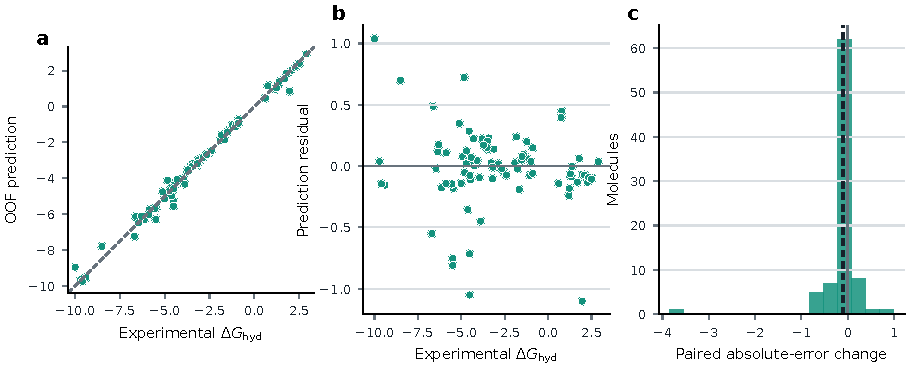
\includegraphics[width=\textwidth]{Supp_Fig1_residuals.pdf}
\end{center}
\noindent\textbf{Supplementary Figure 1 | Molecule-level prediction and residuals.}
\textbf{a}, Confirmatory SolvAI OOF prediction against experiment. \textbf{b}, Signed
residual against experimental hydration free energy. \textbf{c}, Distribution of the
paired absolute-error change relative to the matched structure-only endpoint.

\vspace{1.2em}
\begin{center}
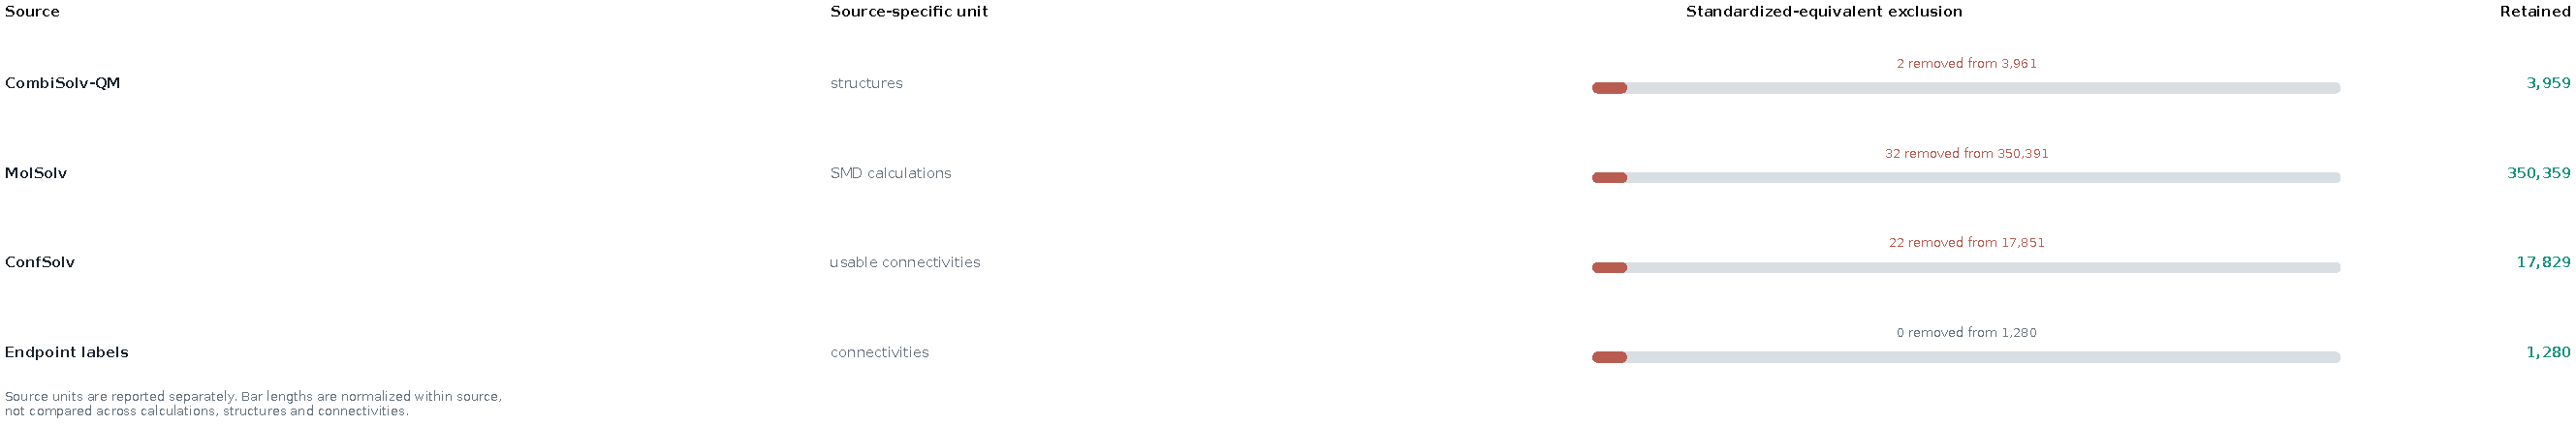
\includegraphics[width=\textwidth]{Supp_Fig2_provenance.pdf}
\end{center}
\noindent\textbf{Supplementary Figure 2 | Source-specific provenance and standardized
identity exclusion.} Counts are shown in their native source units and normalized
only within source. The audit removed standardized benchmark equivalents before the
confirmatory teacher refits; no endpoint experimental label was removed.

\clearpage
\begin{center}
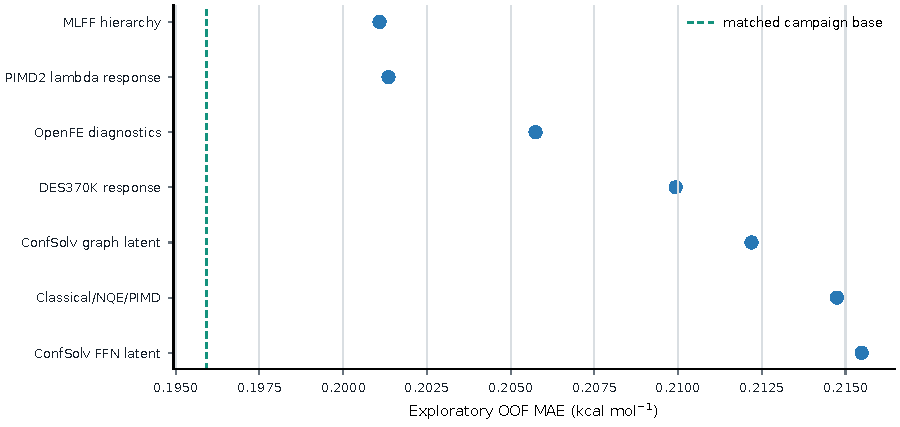
\includegraphics[width=0.88\textwidth]{Supp_Fig3_alternatives.pdf}
\end{center}
\noindent\textbf{Supplementary Figure 3 | Alternative physical-supervision routes.}
Exploratory fixed screens of additional diagnostic, latent and hierarchy features.
The dashed line is the matched campaign response base for those screens. These
experiments were not used to select the confirmatory controls.

\vspace{1.2em}
\begin{center}
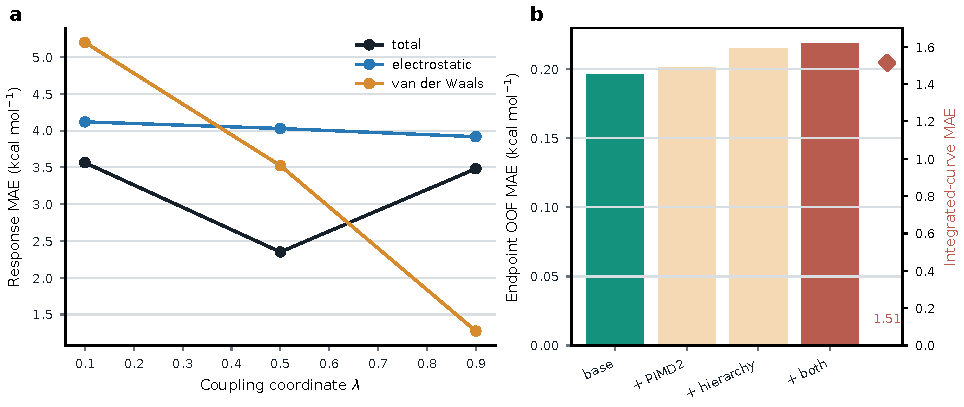
\includegraphics[width=\textwidth]{Supp_Fig4_lambda_response.pdf}
\end{center}
\noindent\textbf{Supplementary Figure 4 | Multi-$\lambda$ response experiment.}
\textbf{a}, OOF response-head error at three coupling states. \textbf{b}, Matched
endpoint consequences and the separately scaled error obtained by direct integration
of the predicted curve.

\clearpage
\begin{center}
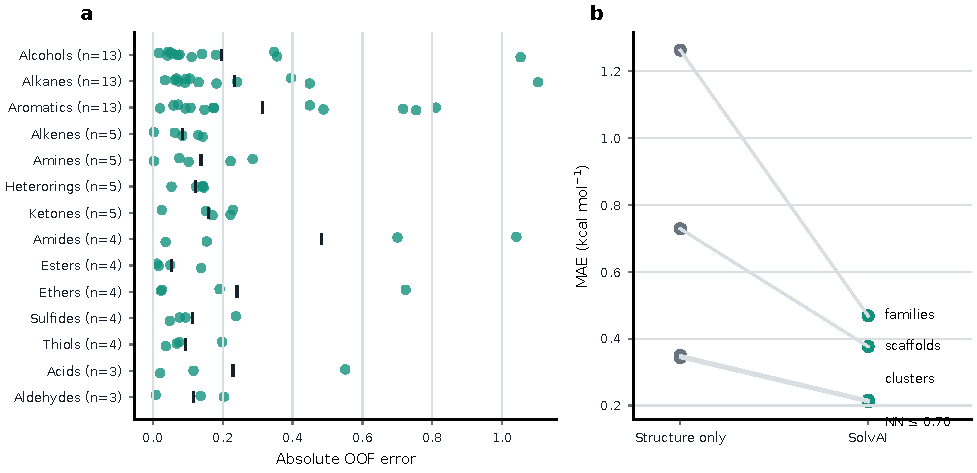
\includegraphics[width=\textwidth]{Supp_Fig5_extrapolation.pdf}
\end{center}
\noindent\textbf{Supplementary Figure 5 | Molecular and chemical-separation errors.}
\textbf{a}, Individual fixed-partition SolvAI errors grouped by diagnostic chemical
family; ticks show family means and labels give sample sizes. \textbf{b}, Matched
structure-only and SolvAI errors under four global separation regimes.

\end{document}
